\section{提案ツールの特長}

\begin{frame}{なぜ,イメージ開発の効率化が必要なのか?}
    下のギャップが,開発を非効率にしている.
    \begin{description}[labelwidth=6.0zw]
        \item[イメージ開発] Dockerfileを作成する.
        \item[動作確認] コンテナ内で行う.
    \end{description}

    \vskip1.0zh
    現状の動作確認の手段
    \begin{enumerate}
        \item 同じベースイメージから起動したコンテナを使う.
        \item 開発中のDockerfileから逐一起動するコンテナを使う.
    \end{enumerate}

    \vskip0.5zh
    どちらも,\textcolor{red!75}{問題あり}.
\end{frame}


\begin{frame}{同じベースイメージから起動したコンテナで\\動作確認しながら,Dockerfileを開発する}
    目的の環境構築とDockerfileの編集作業を同時進行させる.

    → \textcolor{red!75}{開発者の負担が大きい}
    \vskip1.5zh

    \begin{figure}
        \centering
        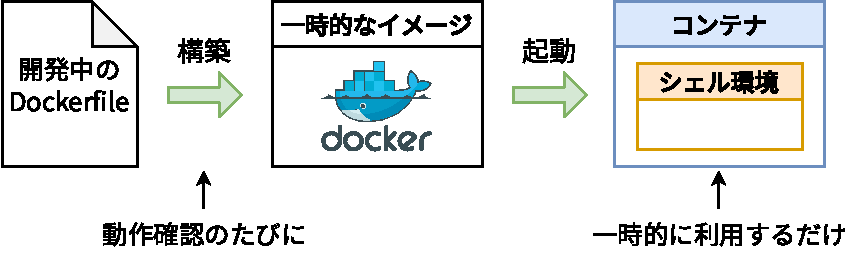
\includegraphics[width=\linewidth]{img/method1.pdf}
    \end{figure}
\end{frame}


\begin{frame}{開発中のDockerfileから逐一起動するコンテナで\\動作確認しながら,Dockerfileを開発する}
    Dockerfileを修正する度に,一時的なイメージを構築する.

    → \textcolor{red!75}{待ち時間が発生する}
    \vskip1.5zh

    \begin{figure}
        \centering
        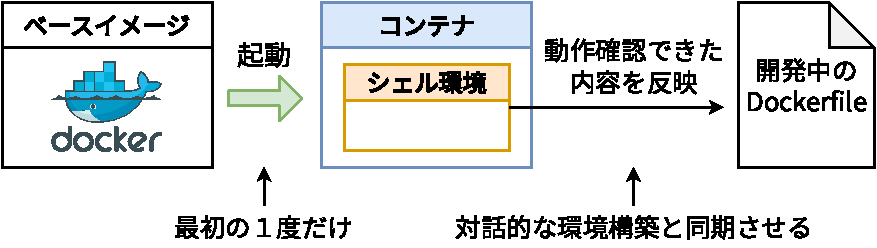
\includegraphics[width=\linewidth]{img/method2.pdf}
    \end{figure}
\end{frame}


\begin{frame}{提案ツールを用いて,Dockerfileを開発すると}
    \begin{figure}
        \centering
        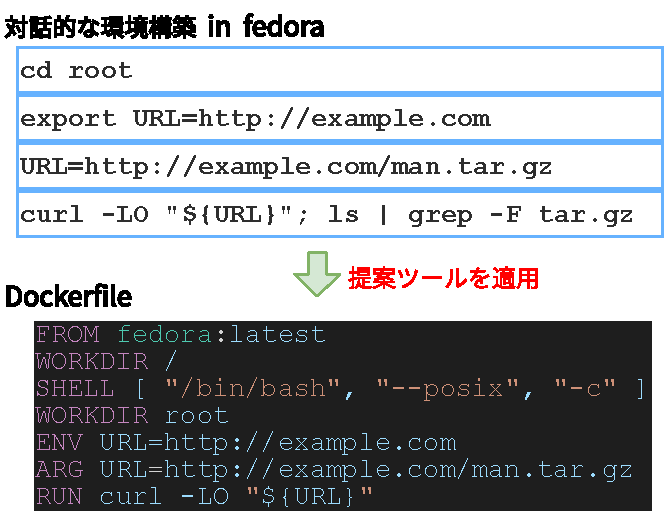
\includegraphics[width=0.95\linewidth]{img/outline.pdf}
    \end{figure}
\end{frame}


\begin{frame}{提案ツールの特長}
    Dockerfileの効率的な開発手法が必要.
    \vskip0.5zh

    \hskip3.0zw
    {\huge $\Downarrow$}
    \vskip0.5zh

    \textcolor{blue!75}{インタラクティブツールとしての側面}

    ユーザがコンテナ内で動作確認しながら環境構築することで,
    \textcolor{red!75}{自動的に}Dockerfileを生成してくれる.
\end{frame}


\begin{frame}{これだけでは優れたDockerfileにはならない}
    \begin{figure}
        \centering
        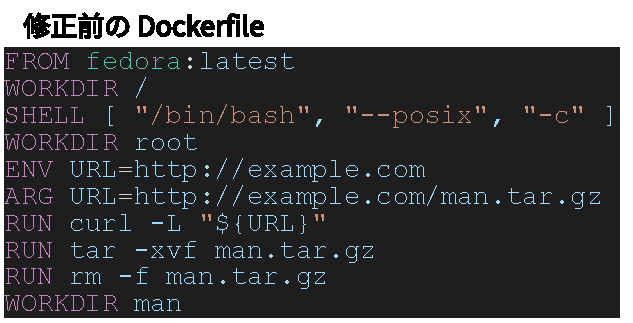
\includegraphics[width=1.02\linewidth]{img/optimize1.pdf}
    \end{figure}

    \begin{tikzpicture}[remember picture]
        \useasboundingbox (0.0, 0.0);
        \begin{scope}[shift={(current page.south west)}]
            \only<2>{\node[probrem] at (6.4, 4.0) {見づらい};}

            \begin{onlyenv}<3>
                \node[callout, callout absolute pointer={(5.6, 4.8)}] at (8.6, 6.6) {絶対パス指定の方がいい};
                \node[callout, callout absolute pointer={(6.4, 3.4)}] at (9.0, 2.0) {集約した方がいい};
                \node[callout, callout absolute pointer={(7.2, 4.2)}] at (9.0, 2.0) {集約した方がいい};
            \end{onlyenv}
        \end{scope}
    \end{tikzpicture}
\end{frame}


\begin{frame}{Dockerfileのリファクタリング・最適化を行ってみる}
    \begin{figure}
        \centering
        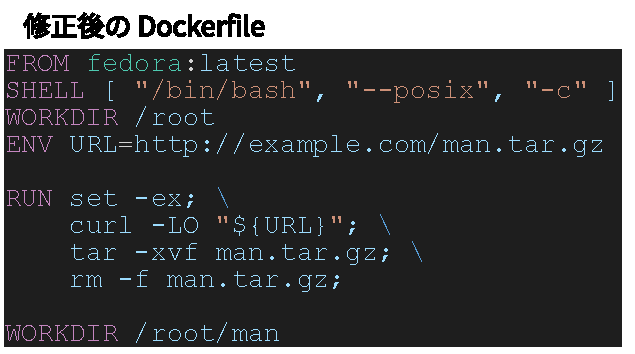
\includegraphics[width=1.02\linewidth]{img/optimize2.pdf}
    \end{figure}
\end{frame}


\begin{frame}{提案ツールの特長}
    \textcolor{blue!75}{インタラクティブツールとしての側面}

    ユーザがコンテナ内で動作確認しながら環境構築することで,
    \textcolor{red!75}{自動的に}Dockerfileを生成してくれる.

    \vskip1.0zh
    \textcolor{blue!75}{リファクタリング・最適化の機能}

    上のようにして生成したDockerfileに,ベストプラクティスに基づいたリファクタリング・最適化を行うことができる.
\end{frame}